\documentclass[letterpaper,12pt]{article}
\usepackage{fancyhdr}
\usepackage{amsmath}
\usepackage{amssymb}
\usepackage{bm}
\usepackage{numprint}
\usepackage[margin=1in]{geometry}
\usepackage{graphicx}
% Random packages from
% http://tex.stackexchange.com/questions/50070/landscape-figure-in-latex
% Necessary for sideways pictures
\usepackage{wrapfig}
\usepackage{lscape}
\usepackage{rotating}
\usepackage{epstopdf}
\usepackage{tablefootnote}
% for word wrap verbatim
\usepackage{listings}
\lstset{
   breaklines=true,
   basicstyle=\ttfamily}
% \pagestyle{fancy}
% \lhead{Jesse Mu}
% \rhead{CSCI339 Term Project}
% One more .. since we're in the abbreviated subdir
\graphicspath{ {../../figures/abbreviated/} {../../figures/} }



\begin{document}

\title{Cluster Analysis: Identifying Parkinson's Disease Subtypes}
\maketitle

\section{Preprocessing}

\subsection{Dataset Description}
951 subjects, 145 metrics, collected 15-4-2012 from Pablo Martinez Mart\'in. Only
19 features used for clustering and/or interpretation.  50 subjects with
missing values of the features to be used in clustering (brought down to 901).
Imputation may be a good idea later on.

\subsection{Selected Features}

Combination of non-motor scale (NMS) symptoms and standard motor symptoms.
Note: PIGD was deleted after 2015-07-16 meeting.

\begin{table}[h]
  \centering
  \begin{tabular}{l|l|l|l}
    Name & Type & Format & Description \\
    \hline
    nms\_d1 & byte & \%8.0g & cardiovascular \\
    nms\_d2 & byte & \%8.0g & sleep/fatigue \\
    nms\_d3 & byte & \%8.0g & mood/cognition \\
    nms\_d4 & byte & \%8.0g & percep/hallucinations \\
    nms\_d5 & byte & \%8.0g & attention/memory \\
    nms\_d6 & byte & \%8.0g & gastrointestinal \\
    nms\_d7 & byte & \%8.0g & urinary \\
    nms\_d8 & byte & \%8.0g & sexual function \\
    nms\_d9 & byte & \%8.0g & miscellaneous \\
    tremor & float & \%9.0g & tremor \\
    bradykin & float & \%9.0g & bradykinesia\tablefootnote{Impaired ability to
    adjust the body's position.} \\
    rigidity & float & \%9.0g & rigidity \\
    axial & float & \%9.0g & axial\tablefootnote{Issues affecting the middle of
    the body.} \\
  \end{tabular}
  \caption{Selected Features and Details}
  \label{tab:selected-features}
\end{table}

\begin{table}[h]
  \centering
  \begin{tabular}{l|l|l|l}
  Name  &       $\mu$ & $\sigma$ & min-max \\
         \hline
nms\_d1&   1.73&  3.35&   0-24 \\
nms\_d2&   8.75&  8.70&   0-48 \\
nms\_d3&   8.68& 11.55&   0-60 \\
nms\_d4&   1.64&  3.86&   0-33 \\
nms\_d5&   5.42&  7.43&   0-36 \\
nms\_d6&   5.53&  6.79&   0-36 \\
nms\_d7&   8.08&  8.94&   0-36 \\
nms\_d8&   3.52&  5.97&   0-24 \\
nms\_d9&   7.13&  7.79&   0-48 \\
tremor&   2.59&  2.58&   0-12 \\
bradykin& 2.40&  1.41&   0-6 \\
rigidity& 2.24&  1.36&   0-6 \\
axial&    3.25&  2.68&   0-12 \\
  \end{tabular}
  \caption{Descriptive Statistics}
  \label{tab:descriptive-statistics}
\end{table}

\section{$k$-means}

$k$-means clustering with $k = 4$ was tried. Statistics for determining the
optimal number of clusters were used, but were inconclusive: results in
Figure~\ref{tab:numclus}. This probably indicates that the data is not very
well clustered. $k = 2, 3$ provided models that were too simplistic. $k = 5$
did not provide any new information, but rather just fragmented existing
groups.

\begin{table}[h]
  \centering
  \caption{caption}
  \label{tab:numclus}
  \begin{tabular}{l|l}
    Criterion & Optimal $k$ \\
    \hline
    Minimum ASW & Inconclusive  \\
    % TODO: Finish this
  \end{tabular}
\end{table}
\begin{table}[h]
  \centering
  \caption{Cluster statistics}
  \label{tab:cluster_stats}
  \begin{tabular}{l|l}
    Cluster & $n$ \\
    \hline
    1 & 189 \\
    2 & 88 \\
    3 & 221 \\
    4 & 406 \\
  \end{tabular}
\end{table}


\subsection{Decision tree}
% \begin{table}[h]
  % \centering
  % \begin{tabular}{l|l|l|l|l|l}
    % $k$ & CP\tablefootnote{Complexity Parameter} & CV Xerror\tablefootnote{10-fold cross
    % validation} & Root Feature &
    % Root Error & Figure \\
    % \hline
    % 4 & 0.0100 & 0.255 & pigd $<$ 2.5 & 0.563 & Figure~\ref{fig:kmeans-dtree-4} \\
  % \end{tabular}
  % \caption{$k$-kmeans decision trees statistics}
  % \label{tab:k-means-dtrees}
% \end{table}

\begin{figure}[h]
  \centering
  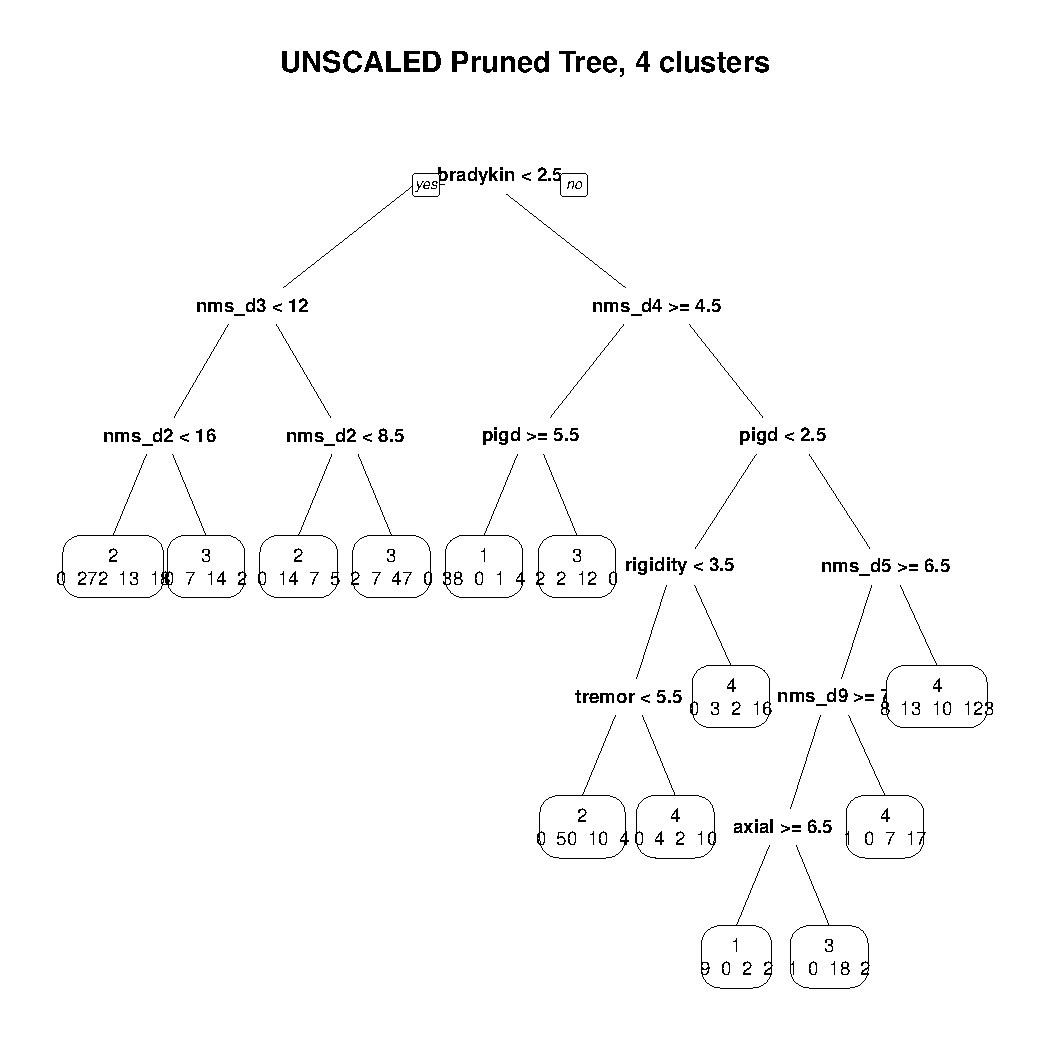
\includegraphics[width=\linewidth]{dtree-kmeans-pruned-unscaled-4.pdf}
  \caption{Decision Tree from $k$-means clustering, 4 clusters}
  \label{fig:kmeans-dtree-4}
\end{figure}

\subsection{Interpretation of Clusters}

\subsubsection{Cluster summaries}

Available in Figure~\ref{fig:kmeans-summaries-4}. Error bar is standard error.

\begin{figure}[h]
  \centering
  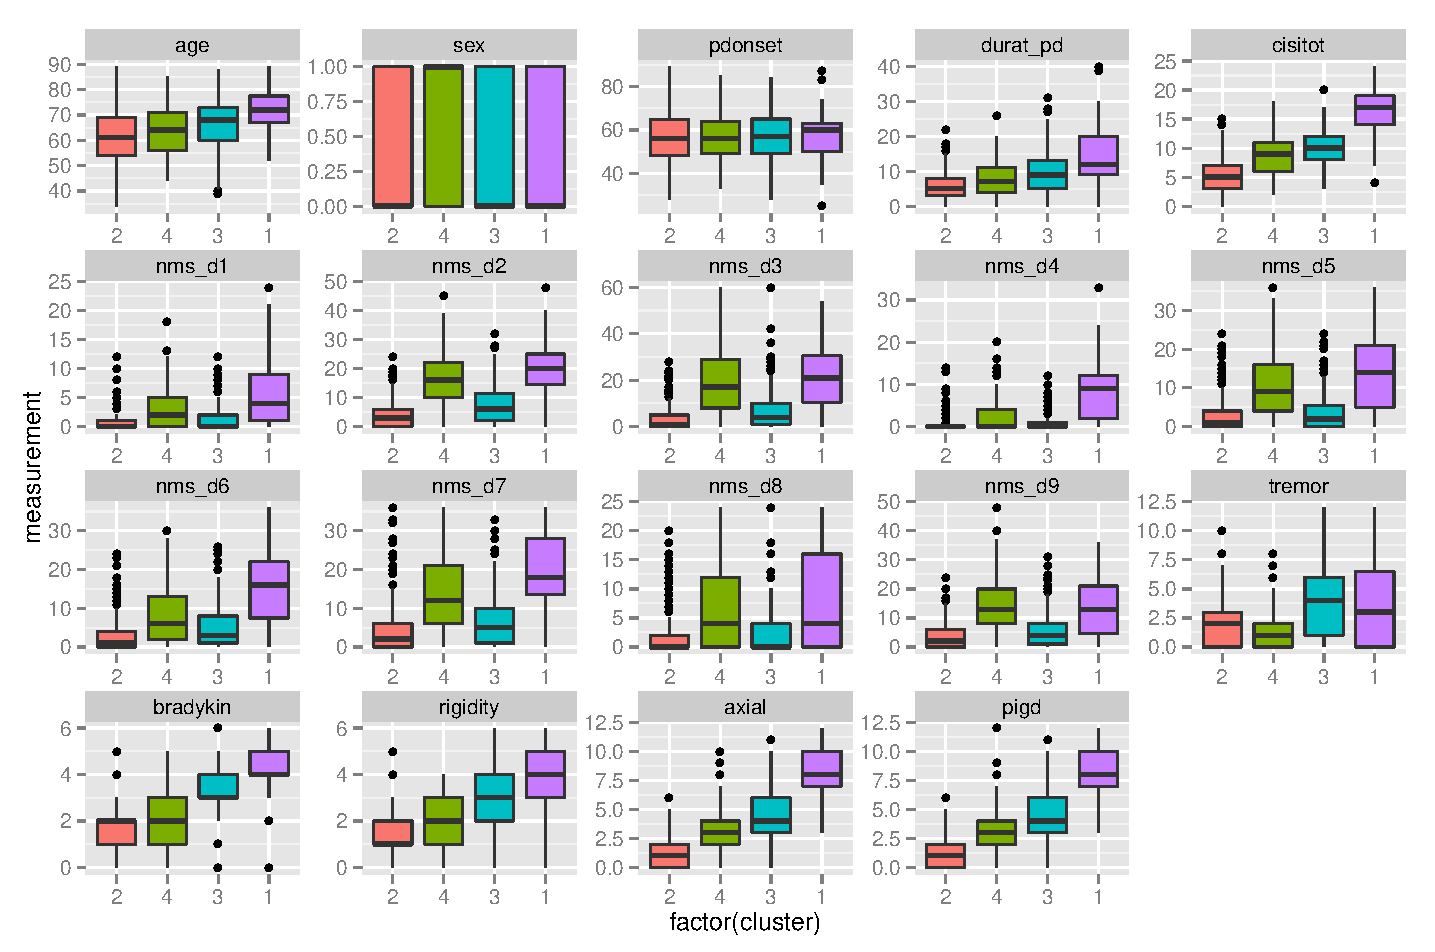
\includegraphics[width=\linewidth]{kmeans-summaries-4.pdf}
  \caption{Cluster Summaries, $k = 4$}
  \label{fig:kmeans-summaries-4}
\end{figure}

\subsubsection{Interpretation}

\subsubsection{Statistical Significance Tests, $k = 4$}
Using one-way ANOVA for multiple means, we reject the null
hypothesis that the means are the same with $p < 0.05$ for every variable
\emph{except} \texttt{pdonset}.

Post-hoc analysis using Tukey's HSD:
\begin{verbatim}
age insignificant differences:
          diff       lwr       upr     p adj
3-1  0.9947808 -1.458184 3.4477455 0.7236845
4-1 -1.2838898 -3.464063 0.8962832 0.4284274
sex insignificant differences:
           diff        lwr        upr      p adj
2-1 -0.05044493 -0.2106093 0.10971941 0.84945412
4-1 -0.09897829 -0.2082638 0.01030726 0.09181043
3-2 -0.12633690 -0.2827741 0.03010026 0.16087872
4-2 -0.04853336 -0.1944676 0.09740091 0.82744866
4-3  0.07780354 -0.0259428 0.18154987 0.21607772
pdonset insignificant differences:
          diff        lwr      upr     p adj
2-1  2.9315777 -0.6232172 6.486373 0.1466742
3-1  1.7136632 -1.0153886 4.442715 0.3699280
4-1  0.7453932 -1.6801637 3.170950 0.8585776
3-2 -1.2179144 -4.6899860 2.254157 0.8033301
4-2 -2.1861845 -5.4251477 1.052779 0.3049434
4-3 -0.9682701 -3.2708860 1.334346 0.7004488
durat_pd insignificant differences:
          diff       lwr        upr        p adj
3-1 -0.7188824 -2.140915  0.7031499 5.624040e-01
cisitot insignificant differences:
          diff         lwr       upr        p adj
3-1  0.4942421  -0.4388731  1.427357 5.228228e-01
nms_d1 insignificant differences:
          diff        lwr        upr        p adj
4-3 -0.3798787 -0.9604053  0.2006478 3.325894e-01
nms_d4 insignificant differences:
          diff        lwr        upr        p adj
4-3 -0.3362459 -0.9972012  0.3247094 5.571480e-01
nms_d5 insignificant differences:
           diff        lwr         upr        p adj
4-3  -0.4117201  -1.743630   0.9201902 8.564409e-01
nms_d8 insignificant differences:
          diff        lwr        upr        p adj
4-3 -0.9953302 -2.1560641  0.1654036 1.220509e-01
nms_d9 insignificant differences:
          diff       lwr        upr      p adj
2-1  0.8708514 -1.297413 3.03911557 0.72966265
4-3 -1.3221920 -2.726684 0.08229967 0.07350641
tremor insignificant differences:
          diff         lwr        upr        p adj
4-1  0.3346105 -0.19270261  0.8619236 3.603863e-01
\end{verbatim}

\subsubsection{Ranked Features by Information Gain}

\begin{table}[h]
  \centering
  \caption{Features ranked by information gain}
  \label{tab:info_gain}
  \begin{tabular}{l|l}
    variable & information gain \\
    \hline
    bradykin      & 0.31574672 \\
    rigidity      & 0.29560018 \\
    nms\_d2      & 0.24218407 \\
    cisitot      & 0.22920103 \\
    axial      & 0.22780750 \\
    nms\_d3      & 0.20480570 \\
    nms\_d9      & 0.15782743 \\
    nms\_d7      & 0.15290569 \\
    nms\_d5      & 0.14454931 \\
    nms\_d6      & 0.14025139 \\
    nms\_d1      & 0.13212756 \\
    tremor      & 0.10937168 \\
    nms\_d4      & 0.10710526 \\
    nms\_d8      & 0.10005480 \\
    durat\_pd      & 0.02876190 \\
    age      & 0.02346158 \\
    sex      & 0.00000000 \\
    pdonset      & 0.00000000 \\
  \end{tabular}
\end{table}

\subsubsection{Correlation Plots}

Figure~\ref{fig:corrplots}.

\begin{figure}[h]
  \centering
  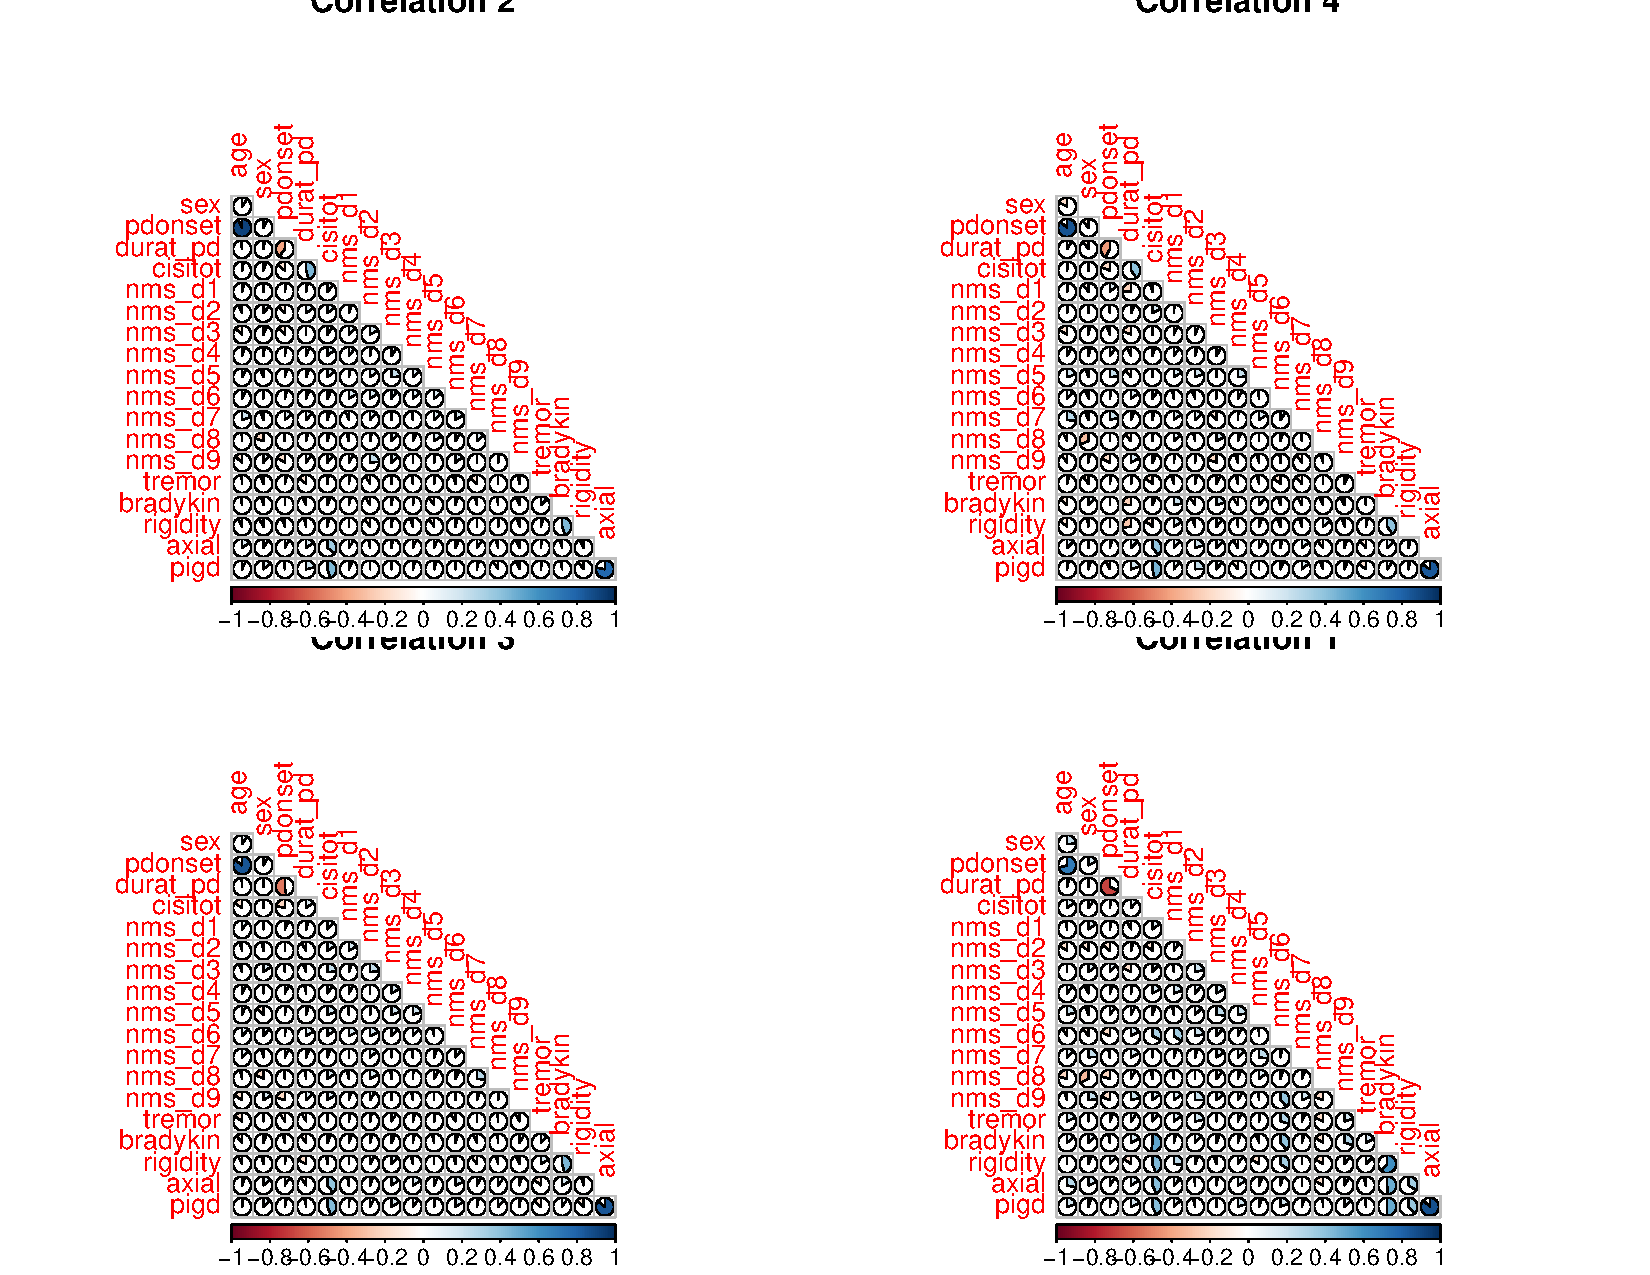
\includegraphics[width=\linewidth]{corrplots.pdf}
  \caption{Correlation plots}
  \label{fig:corrplots}
\end{figure}

\subsubsection{One vs all decision trees}

Figures~\ref{fig:1va},~\ref{fig:2va},~\ref{fig:3va},~\ref{fig:4va}.

\begin{figure}[h]
  \centering
  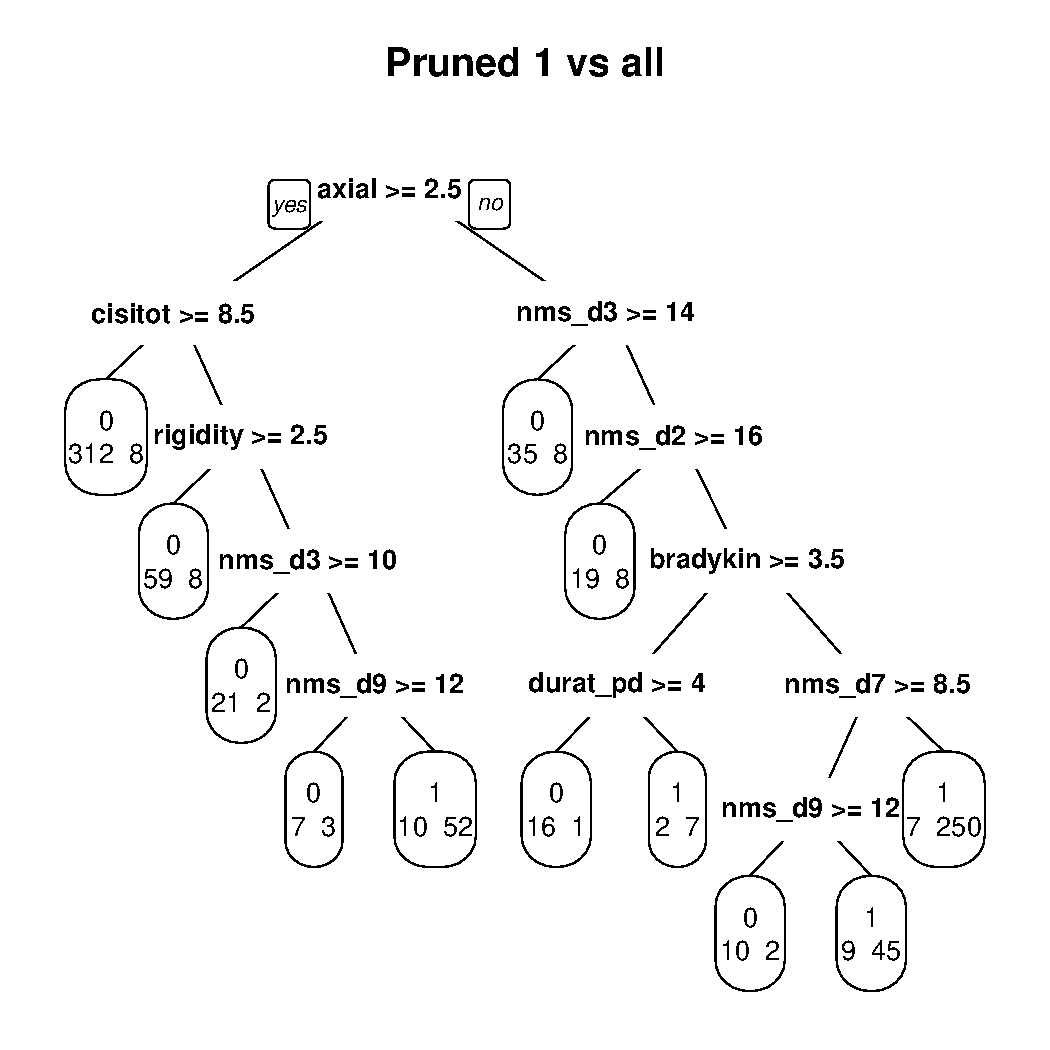
\includegraphics[width=\linewidth]{dtree-1va-pruned.pdf}
  \caption{Cluster 1 vs all}
  \label{fig:1va}
\end{figure}

\begin{figure}[h]
  \centering
  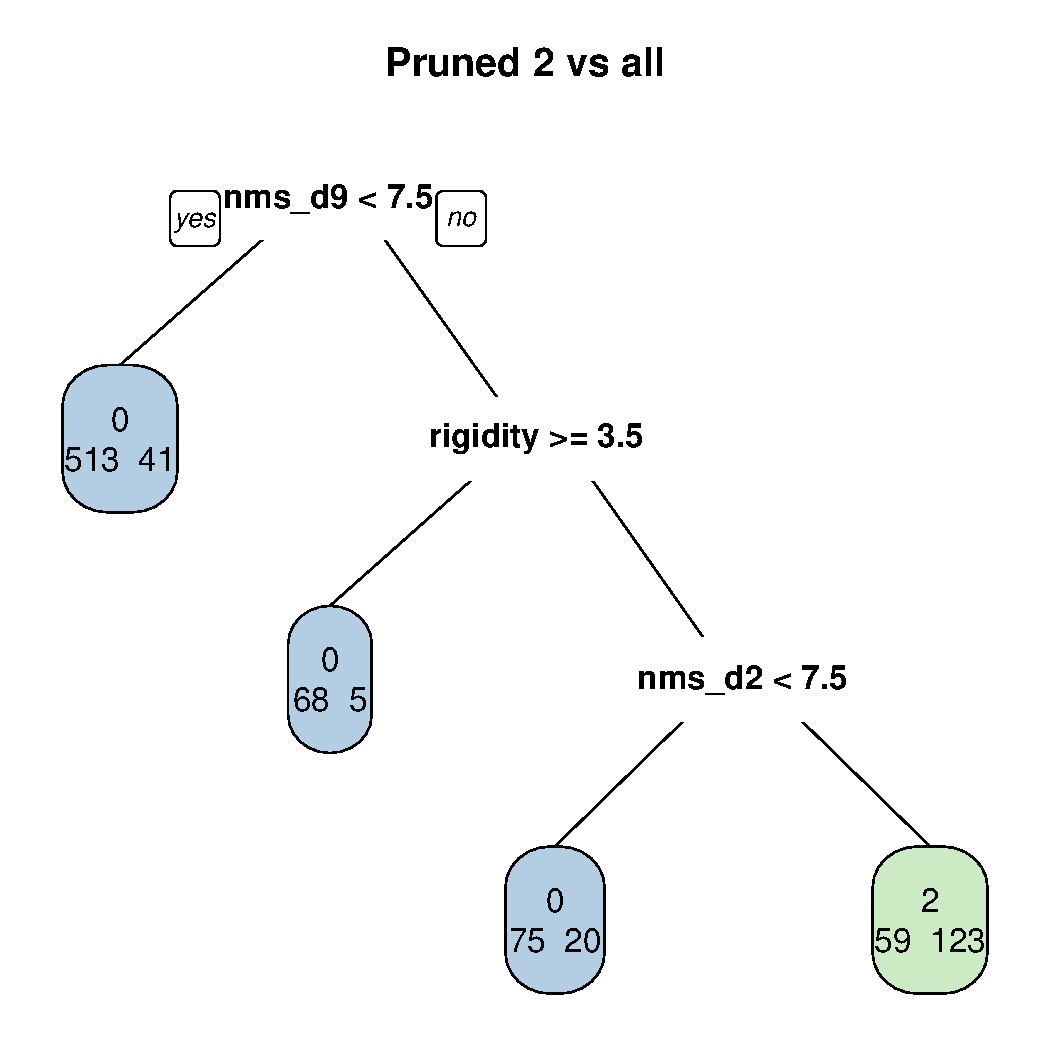
\includegraphics[width=\linewidth]{dtree-2va-pruned.pdf}
  \caption{Cluster 2 vs all}
  \label{fig:2va}
\end{figure}
\begin{figure}[h]
  \centering
  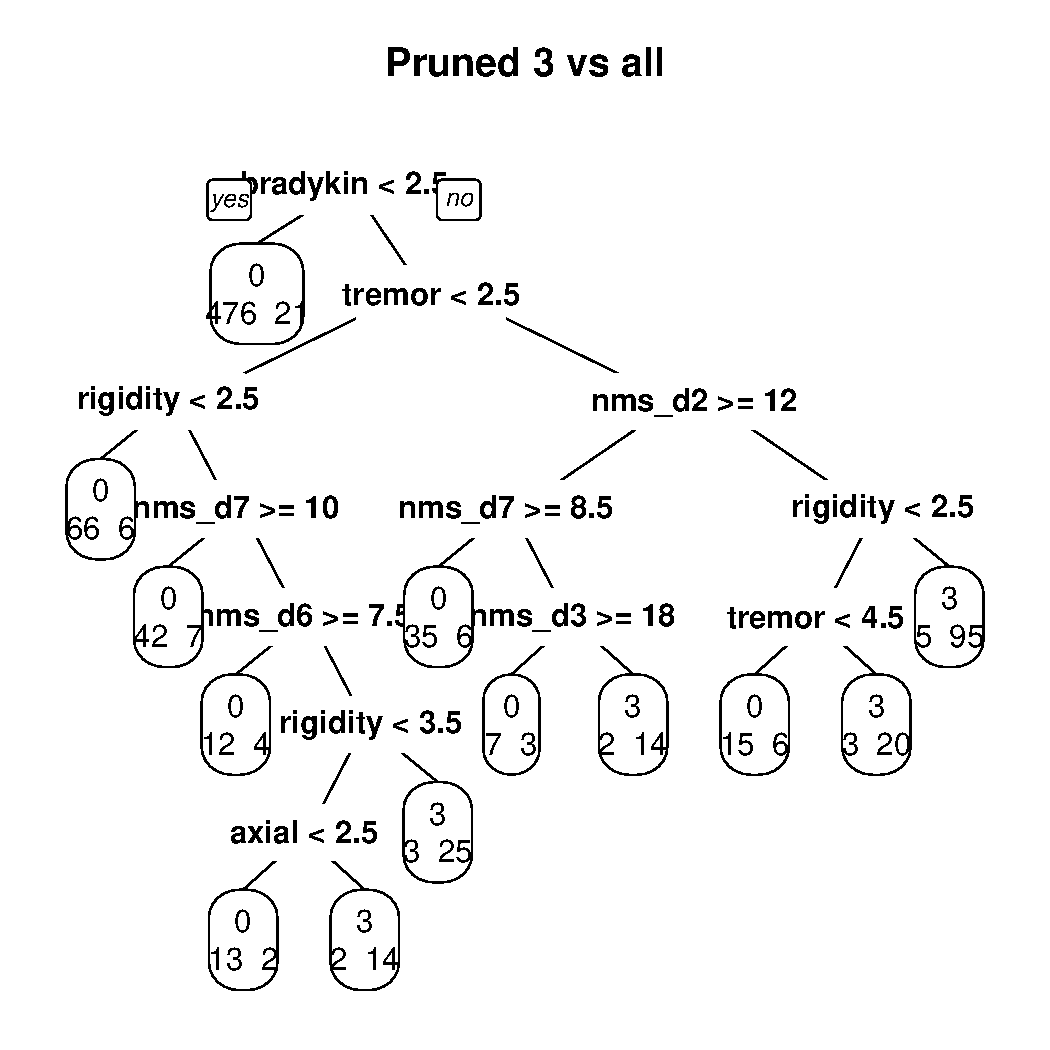
\includegraphics[width=\linewidth]{dtree-3va-pruned.pdf}
  \caption{Cluster 3 vs all}
  \label{fig:3va}
\end{figure}

\begin{figure}[h]
  \centering
  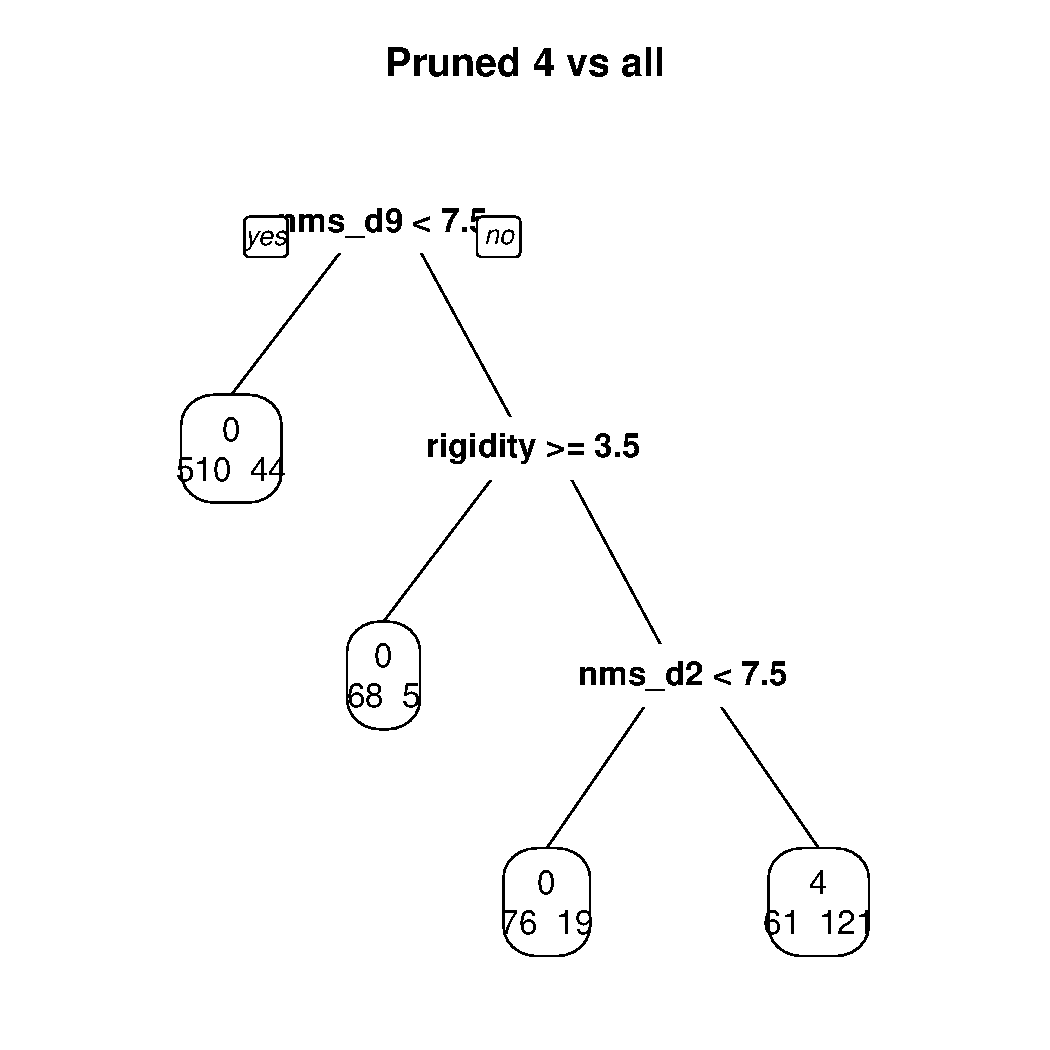
\includegraphics[width=\linewidth]{dtree-4va-pruned.pdf}
  \caption{Cluster 4 vs all}
  \label{fig:4va}
\end{figure}
\section{Other Work}

\subsection{Bayesian Networks on Cluster 1}

Figures~\ref{fig:bnet-gs},~\ref{fig:bnet-hc}, and~\ref{fig:bnet-mmhc} show various
learning algorithms.

\begin{figure}[h]
  \centering
  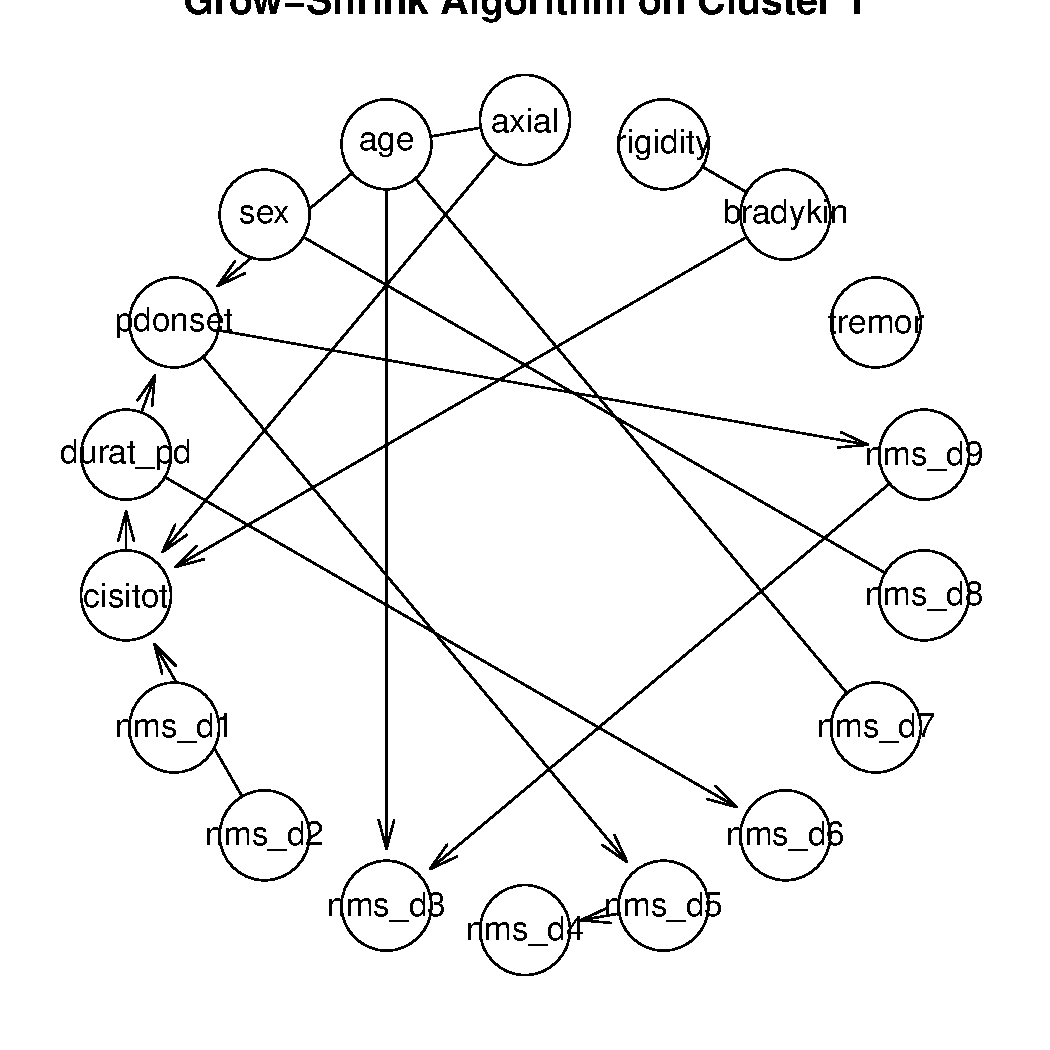
\includegraphics[width=\linewidth]{clus1-bnet-gs.pdf}
  \caption{Grow Shrink Algorithm}
  \label{fig:bnet-gs}
\end{figure}

\begin{figure}[h]
  \centering
  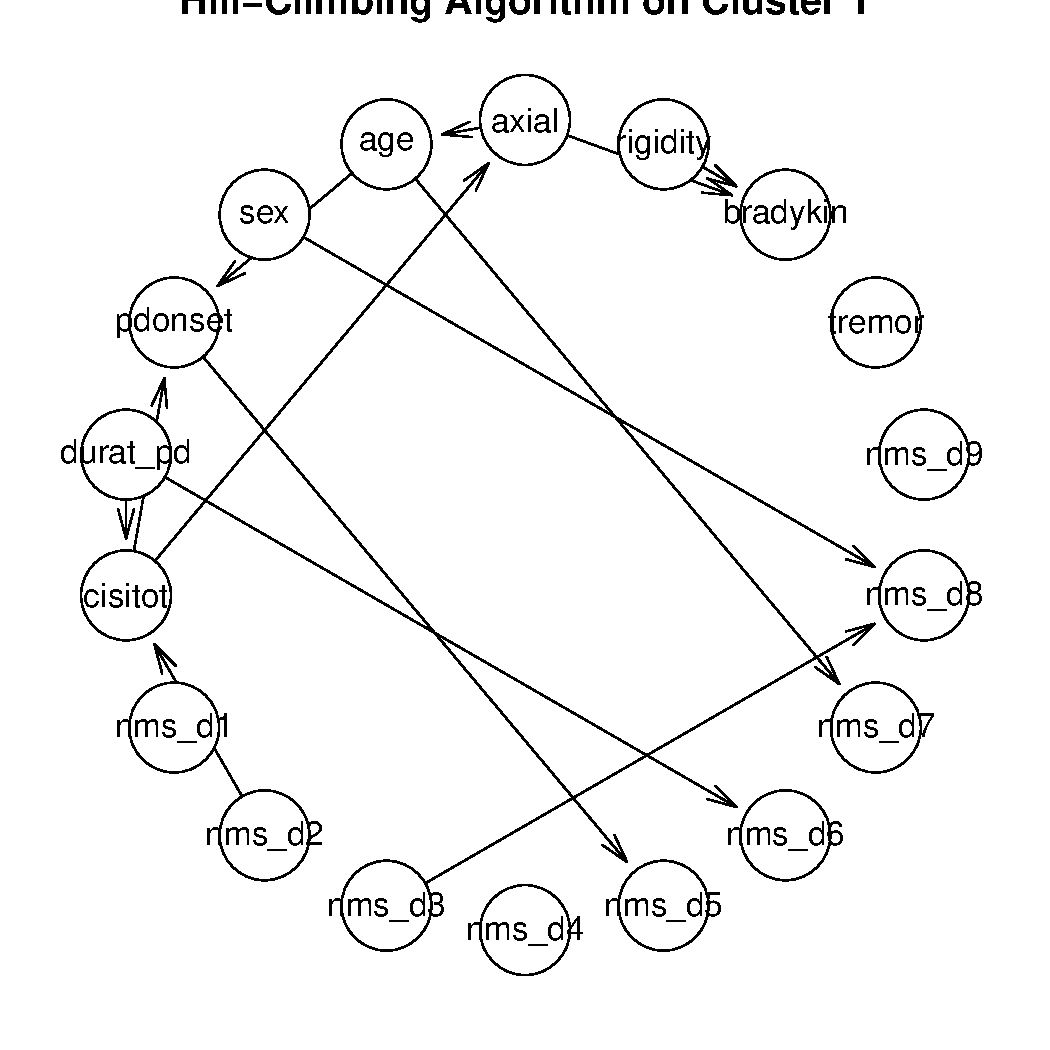
\includegraphics[width=\linewidth]{clus1-bnet-hc.pdf}
  \caption{Hill Climbing Algorithm}
  \label{fig:bnet-hc}
\end{figure}

\begin{figure}[h]
  \centering
  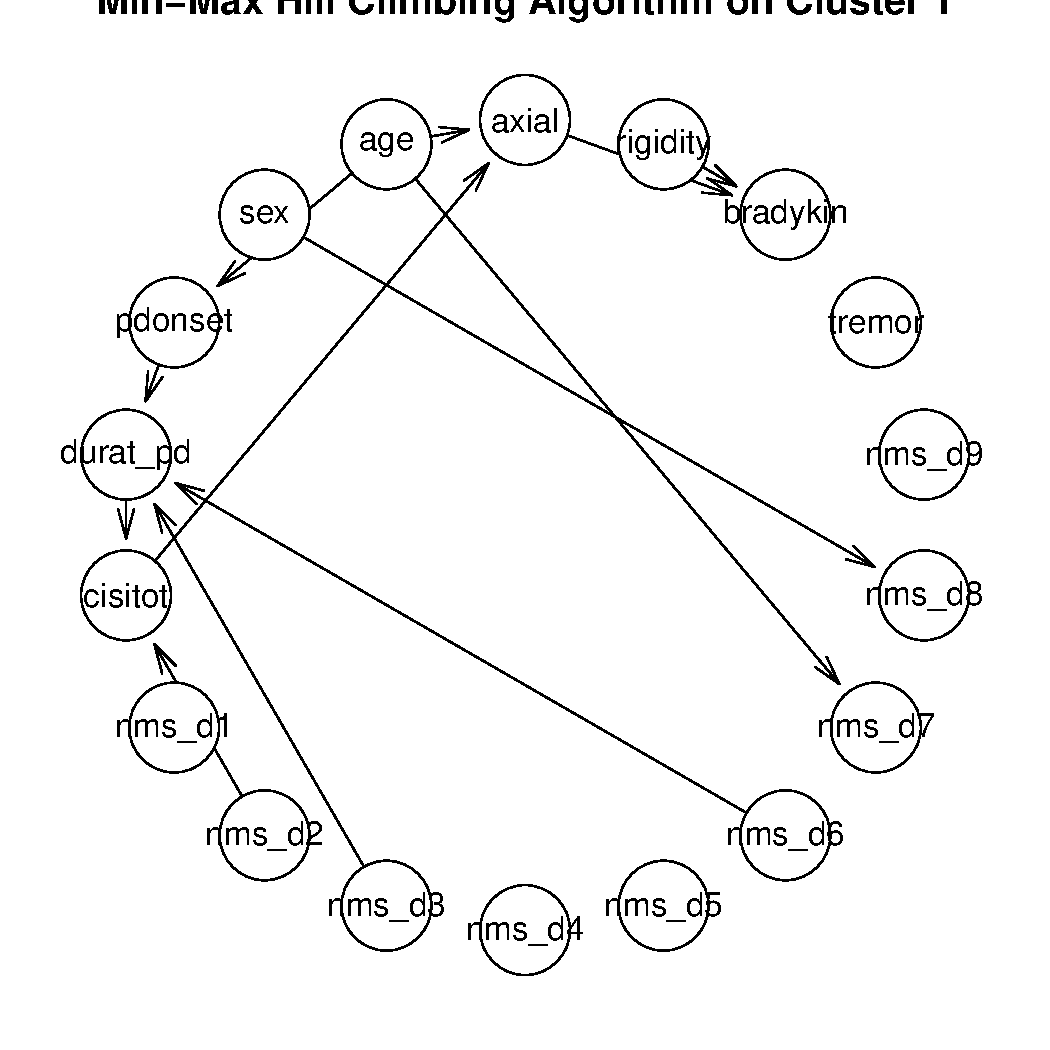
\includegraphics[width=\linewidth]{clus1-bnet-mmhc.pdf}
  \caption{Min-Max Hill Climbing Algorithm}
  \label{fig:bnet-mmhc}
\end{figure}

\subsection{$k$-means on Cluster 1}

Figures~\ref{fig:c1-summaries-2},~\ref{fig:c1-summaries-3},
and~\ref{fig:c1-summaries-4}.

\begin{figure}[h]
  \centering
  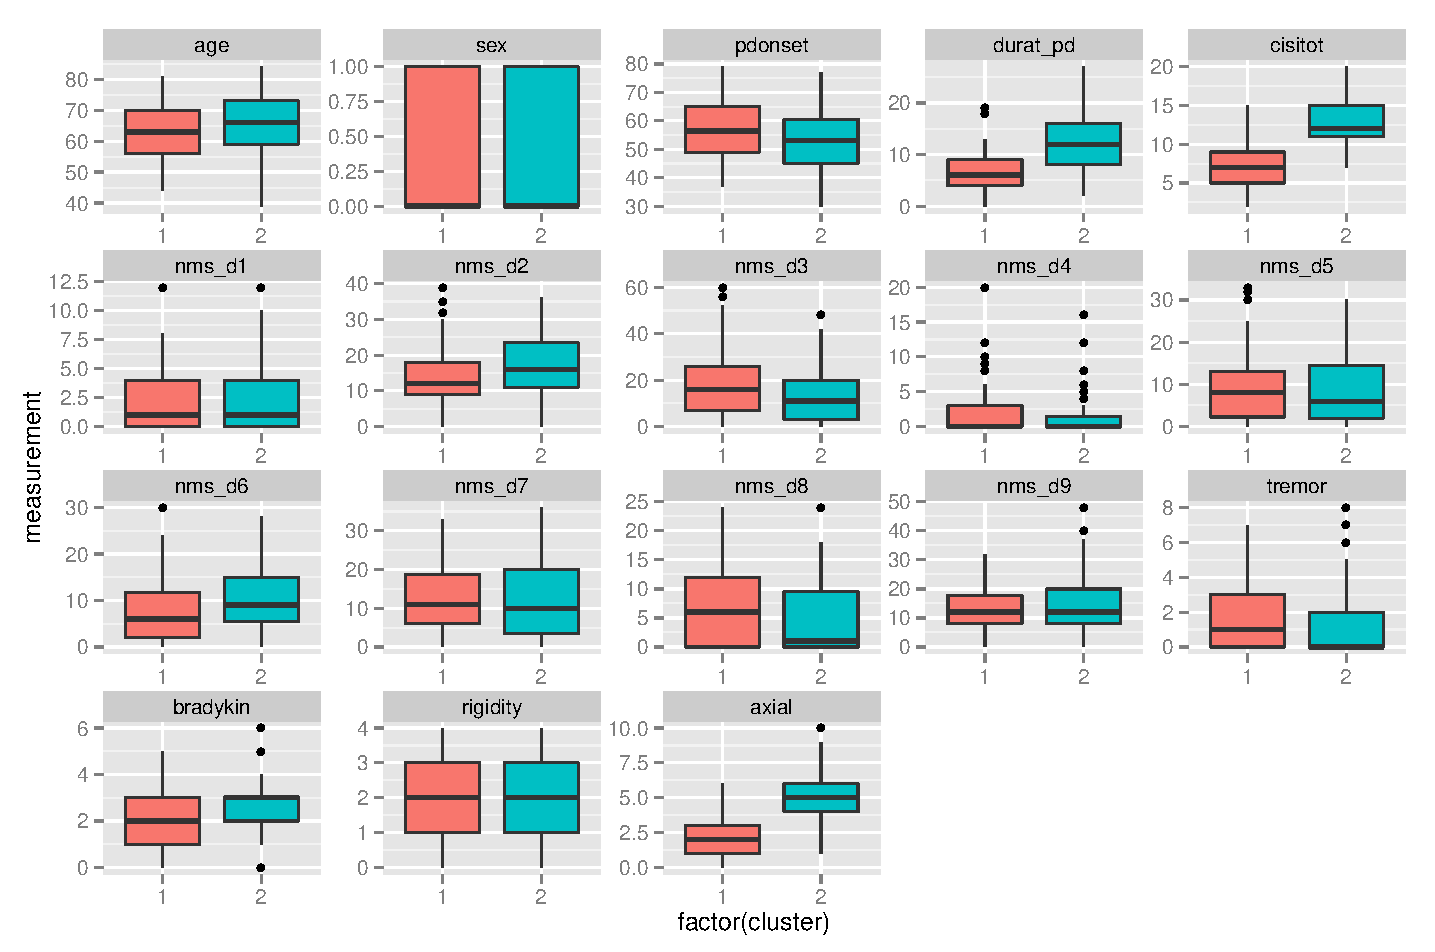
\includegraphics[width=\linewidth]{c1-summaries-2.pdf}
  \caption{$k = 2$}
  \label{fig:c1-summaries-2}
\end{figure}
\begin{figure}[h]
  \centering
  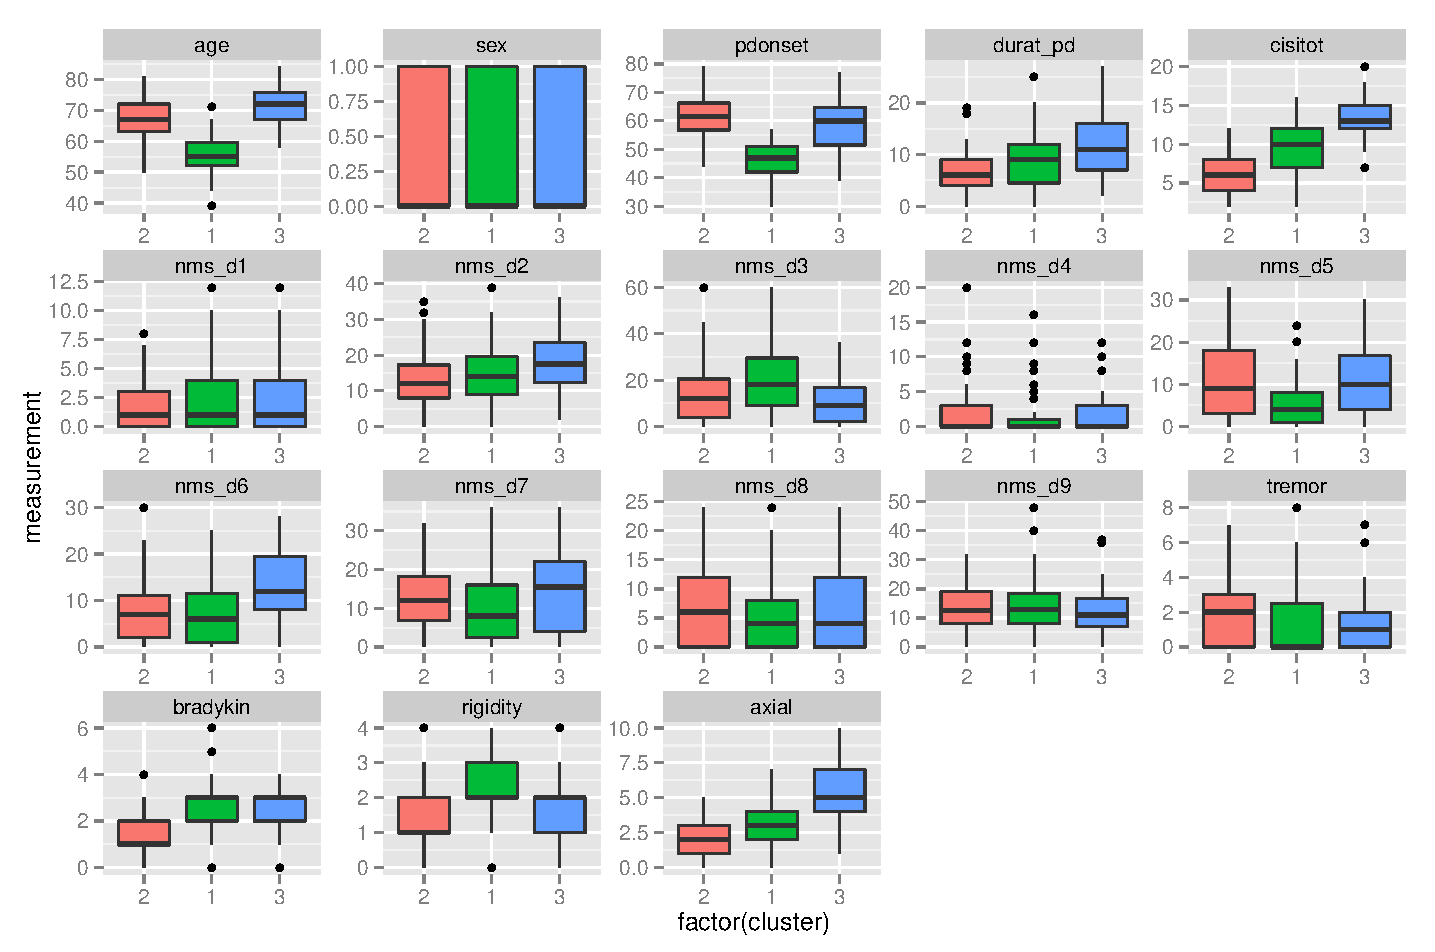
\includegraphics[width=\linewidth]{c1-summaries-3.pdf}
  \caption{$k = 3$}
  \label{fig:c1-summaries-3}
\end{figure}
\begin{figure}[h]
  \centering
  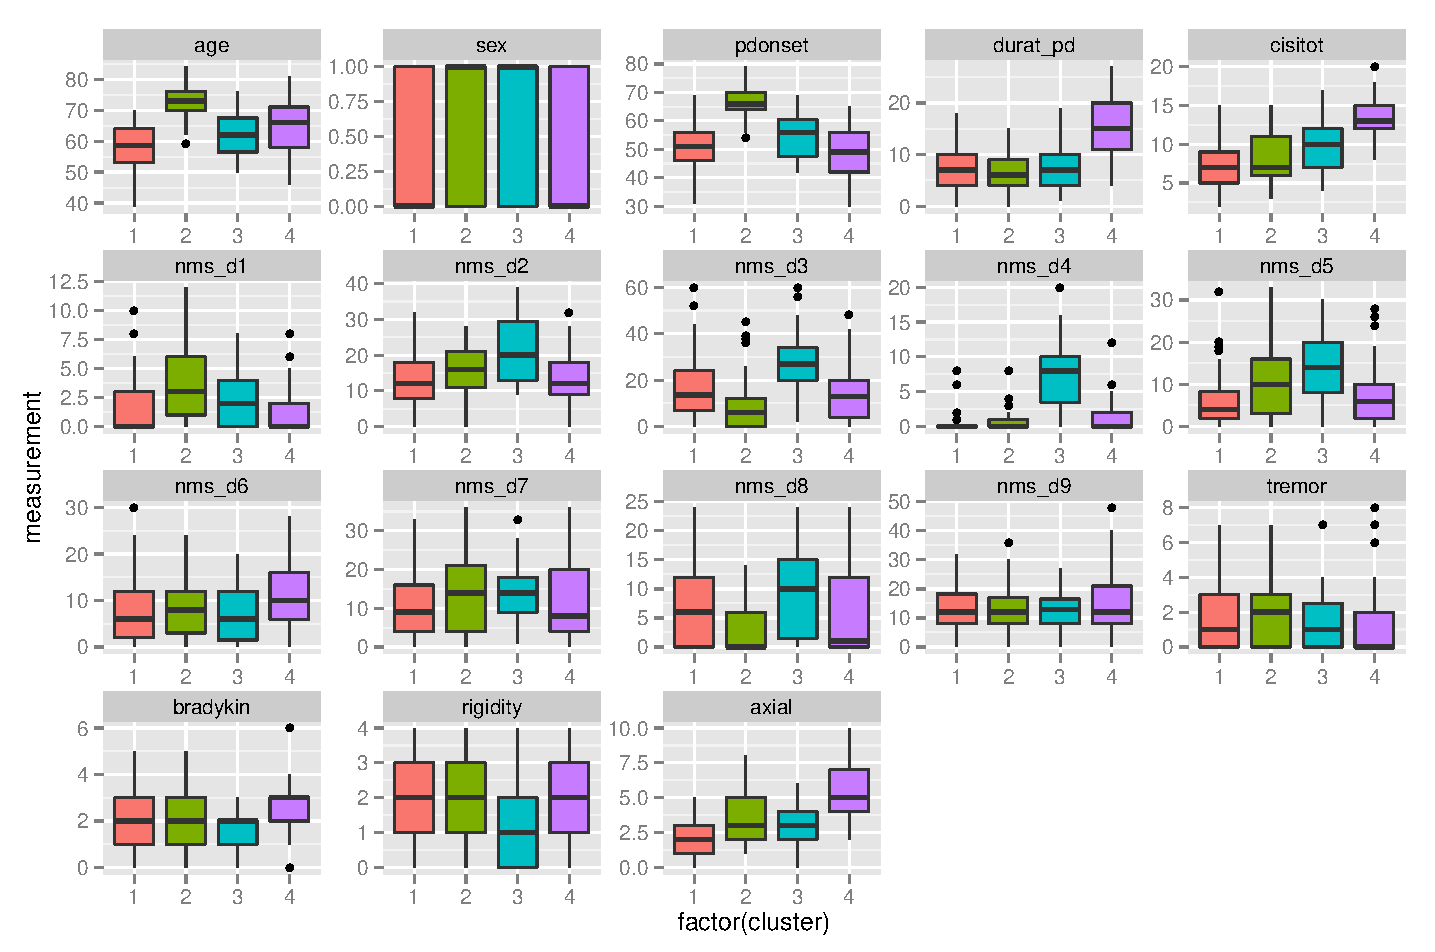
\includegraphics[width=\linewidth]{c1-summaries-4.pdf}
  \caption{$k = 4$}
  \label{fig:c1-summaries-4}
\end{figure}

\end{document}
